\documentclass{standalone}
\usepackage{tikz}
\usetikzlibrary{3d}
\usetikzlibrary{arrows}
\usepackage{transparent}
\begin{document}
\begin{tikzpicture}[x={(0.866cm,-0.5cm)}, y={(0.866cm,0.5cm)}, z={(0cm,1cm)}, scale=1.0,
    %Option for nice arrows
    >=stealth, %
    inner sep=0pt, outer sep=2pt,%
    axis/.style={very thick,->},
    wave/.style={thick,color=#1,smooth},
    polaroid/.style={fill=black!60!white, opacity=0.01},
]

\filldraw[polaroid] (0,-4,-3) -- (0,-4,3) -- (0,4,3) -- (0,4,-3) -- (0,-4,-3);

	\node[canvas is zy plane at x=0,above right,opacity=0.1] (foto) at (0,-4.1,-3.1) {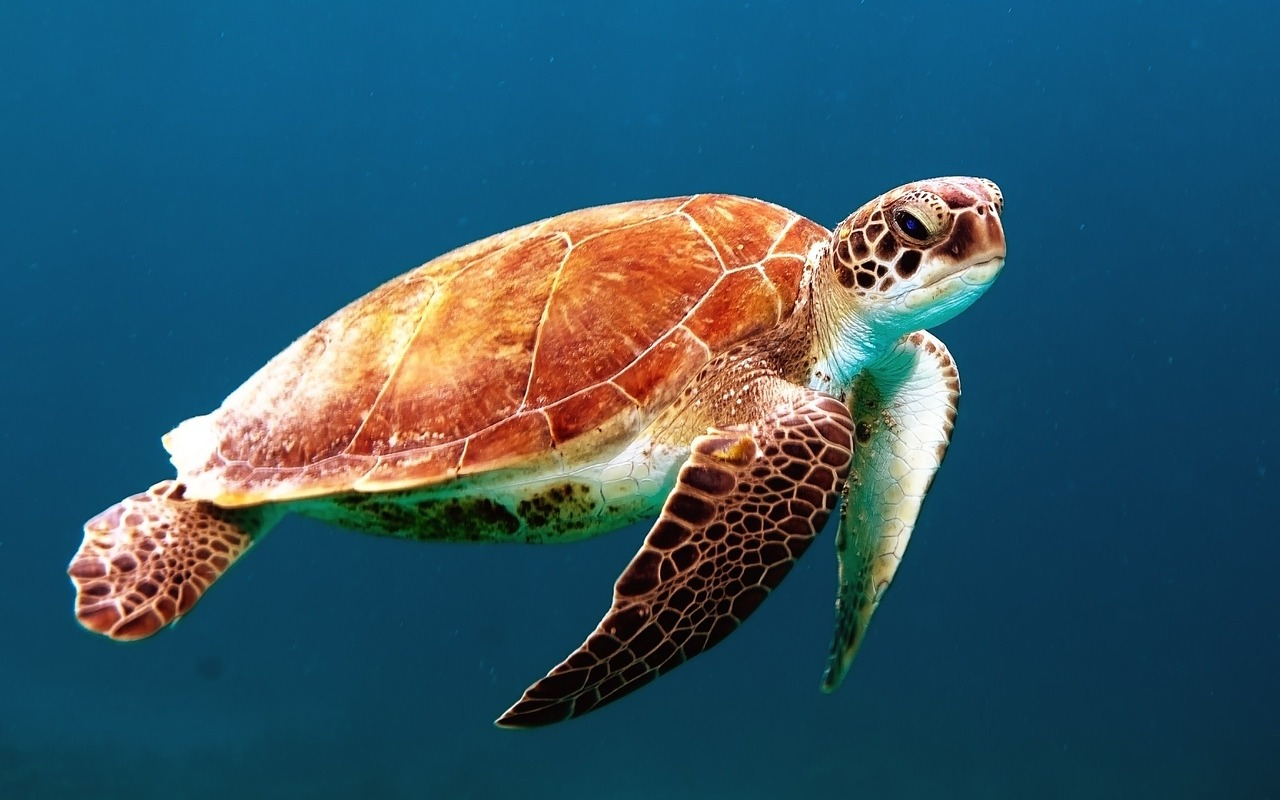
\includegraphics[width=8cm,height=6cm,angle=270]{turtle.jpg}};
\draw[red, dashed]   (0, -4, -3) -- (8,0, 0);
\draw[red, dashed,opacity=0.2]   (4, 2, -1.5) -- (0,4, -3);	
\draw[red, dashed]   (4, 2, -1.5) -- (8,0, 0);
\draw[red, dashed]   (0, -4, 3) -- (8,0, 0);
\draw[red, dashed]   (0, 4, 3) -- (8,0, 0);

\filldraw[polaroid] (4,-2,-1.5) -- (4,-2,1.5) -- (4,2,1.5) -- (4,2,-1.5) -- (4,-2,-1.5);

\node[canvas is zy plane at x=0,above right,opacity=0.3] (foto) at (4,-2 .1,-1.55) {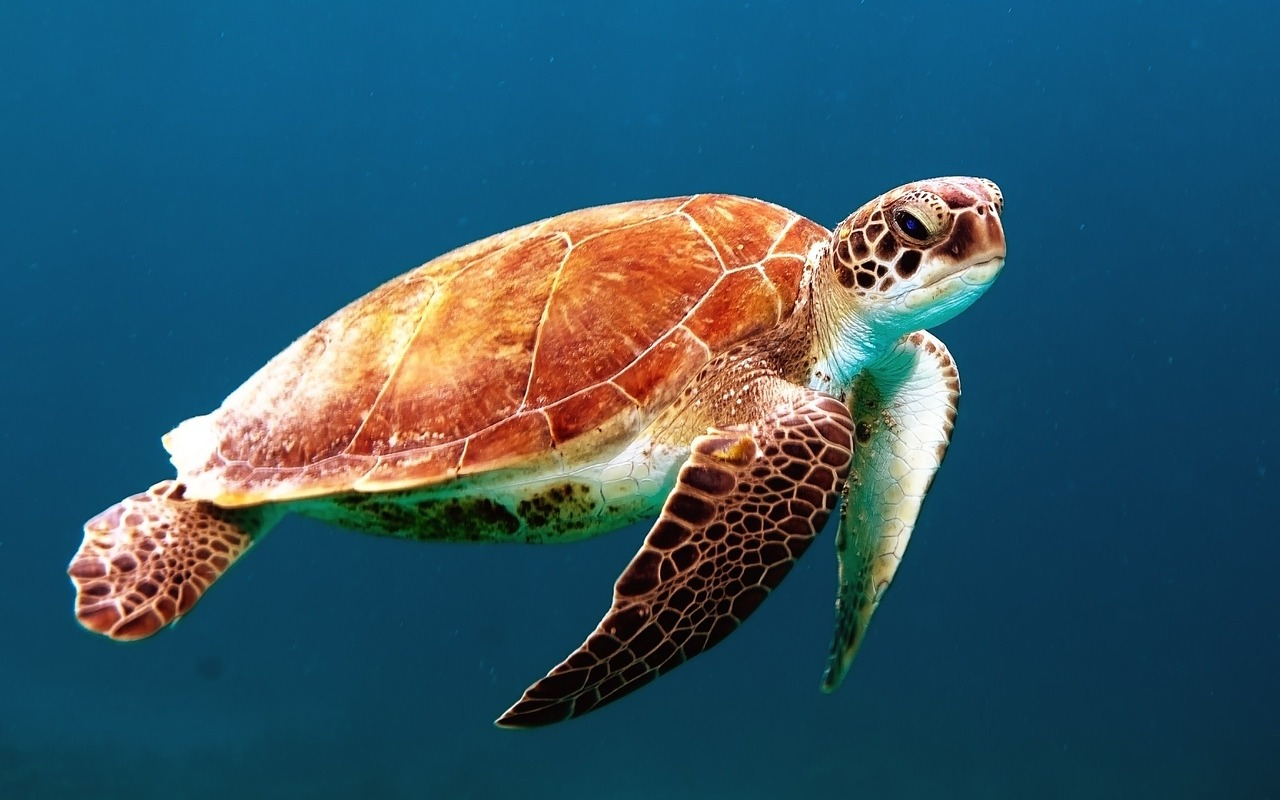
\includegraphics[width=4cm,height=3cm,angle=270]{turtle.jpg}};

    % Colors
    \colorlet{darkgreen}{green!50!black}
    \colorlet{lightgreen}{green!80!black}
    \colorlet{darkred}{red!50!black}
    \colorlet{lightred}{red!80!black}

    % Frame
    \coordinate (O) at (0, 0, 0);
    \draw(8,0,0) -- (0, 0,   0);
    \draw(8,-2.5,0) -- (8, 2, 0);
    \draw(0,-4.5,0) -- (0, 4.5, 0);
	\draw[axis] (8,0,0) -- (7, 0,   0) node [above] {\textbf{z}};
    \draw[axis] (8,0,0) -- (8,  1, 0) node [right] {\textbf{x}};
    \draw[axis] (8,0,0) -- (8,  0,   -1) node [below] {\textbf{y}};
    
    \draw[dashed,ultra thick,->, cyan] (4,-2.5,0) -- (4,  2.5, 0) node [right] {\textbf{x}};
    \draw[dashed,ultra thick,->, cyan] (4,0,2) -- (4,  0,   -2) node [below] {\textbf{y}};

    \draw[dashed,ultra thick,->, gray] (4,-2,1.5) -- (4,  2.5, 1.5) node [right] {\textbf{u}};
	\draw[dashed,ultra thick,->, gray] (4,-2,1.5) -- (4,  -2,   -2) node [below] {\textbf{v}};
	
	
    \draw[gray] (4,-2,0.5) -- (4, 1, 0.5);
    \draw[gray] (4,-2,0.6) -- (4, 0.9, 0.6);
    \draw[gray] (4,1,1.5) -- (4, 1, 0.5);
    \draw[gray] (4,0.9,1.5) -- (4, 0.9, 0.6);
    
    \foreach \i in {-2,-1.9,...,1}
    {
    	\draw[gray] (4,\i,0.6) -- (4, \i, 0.5);
    }

    \foreach \i in {1.5,1.4,...,0.5}
	{
	\draw[gray] (4,1,\i) -- (4,0.9, \i);
	}
    
	\draw[dashed,ultra thick,->, gray] (4,-2,1.5) -- (4,  -2,   -2) node [below] {\textbf{v}};
	\draw[ultra thick, red] (8,0,0) -- (4,  0.95, 0.55);
	\draw[ultra thick, red,opacity=0.8] (3.2,  1.15, 0.65) -- (0,  2*0.95, 2*0.55);
	\draw[ultra thick, red,opacity=0.2] (4,  0.95, 0.55) -- (0,  2*0.95, 2*0.55);
	\draw[ line width=2mm, red,opacity=0.8, ->] (0,  2*0.95, 0) -- (0,  2*0.95, 2*0.55);
	\draw[ line width=0.8mm, red,opacity=0.8, ->] (4,  0.95, 0) -- (4,  0.95, 0.55);
    \draw[thick,dashed] (-2,0,0) -- (O);
    
	\draw[thick,<->,darkred] (4,-2.5,0) -- (8, -2.5, 0) node[midway,fill=white,left]{F};
	\node[gray] at (4,1.5,0.3){(u,v)};
    % monochromatic incident light with electric field
   % \draw[wave=blue, opacity=0.7, variable=\x, samples at={-2,-1.75,...,0}]
    %    plot (\x, { cos(1.0*\x r)*sin(2.0*\x r)}, {§§ sin(1.0*\x r)*sin(2.0*\x r)})
    %    plot (\x, {-cos(1.0*\x r)*sin(2.0*\x r)}, {-sin(1.0*\x r)*sin(2.0*\x r)});








	

    %\draw[thick, <->] (12, -1.5,-0.5) -- (12, -1.5, 0.5); %Polarization direction


\end{tikzpicture}
\end{document}